%%
%% cap3.tex
%% 
%% Made by Carlos Calcaneo Roldan
%% Login   <calcaneo@jogrant>
%% 
%% Started on  Mon Jul 22 15:03:25 2019 Carlos Calcaneo Roldan
%% Last update Time-stamp: <2020-jul-29.miércoles 19:05:05 ()>
%%
%%%%%%%%EL TExto Comienza abajo de aquí! 
\chapter{Halos de Materia Oscura}
\setcounter{equation}{0}

\noindent Con la intención de conocer y diferenciar diferentes cosmologías, en nuestro estudio de los halos de materia oscura, optamos por realizar fue una variedad de simulaciones de materia oscura. Desde simulaciones con cosmologías de Universos planos ($\Omega = 1$), asi como cosmologías  de universos con densidades sub-criticas ($\Omega < 1$) y super-criticas ($\Omega > 1$).

\section[Cosmología Plana \texorpdfstring{$\Omega = 1$}{Omega = 1}]{Cosmología Plana \texorpdfstring{$\Omega = 1$}{Omega = 1}}

\noindent Comenzaremos con un estudio de las cosmologías planas (aquellas donde las densidades sean $\Omega = 1$). Estudiaremos 3 cosmologías planas, empezando con las que tiene las densidades mas aceptadas de nuestro Universo ($\Omega_\lambda = 0.691$, $\Omega_0 = 0.309$  \cite{2020A&A...641A...1P}). Luego pasaremos nuestra atención a estudiar los efectos que hay con las densidades invertidas ($\Omega_\lambda = 0.309$, $\Omega_0 = 0.691$) y para terminar con las cosmologías planas veremos los efectos en un Universo con densidades iguales ($\Omega_\lambda = 0.5$, $\Omega_0 = 0.5$).

 \subsection{Universo con cosmología  \texorpdfstring{$\Omega_\lambda = 0.691$, $\Omega_0 = 0.309$ }{Omega lambda = 0.691, Omega 0 = 0.309}  }

 En la evolución de este Universo, la materia comienza a agruparse lentamente en lo que llamamos halos. En un principio la materia parece una nube difusa sin estructuras internas, después de un tiempo en el que se esta agrumando, pequeñas estructuras de materia se empiezan a formar. Las primeras estructuras son pocas como se aprecia en la figura \ref{fig:EvoNumTotHalos}. Las estructuras tardan tiempo en aparecer y eventualmente hay un aumento acelerado en la cantidad halos que se forman y mas hacia al presente vemos un pico donde empiezan a disminuir el total de halos.

\begin{figure}[ht!]
    \centering
    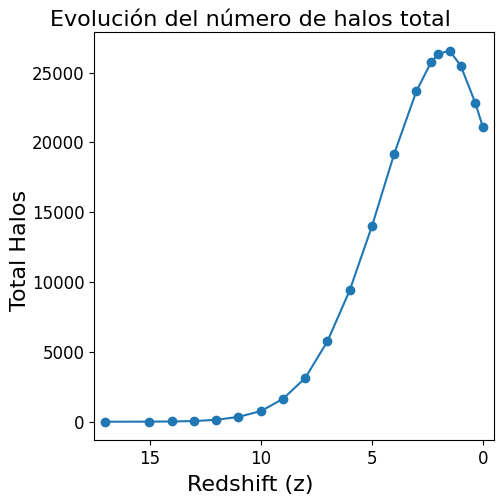
\includegraphics[scale = 0.5]{RunCanonica/TotalHalos_RunCanonica.png}
    \caption[Evolución del número de halos en un Universo $\Omega_\lambda = 0.691 $, $\Omega_0 = 0.309$]{\footnotesize Se muestra el numero de halos y como cambia la cantidad conforme evoluciona el Universo en una cosmología $\Omega_\lambda = 0.691 $ y $\Omega_0 = 0.309$.}
    \label{fig:EvoNumTotHalos}
\end{figure}

En la figura \ref{fig:MassDistCanonRunSep} y \ref{fig:MassDistCanonRun} podemos observar que aunque disminuyen la cantidad de halos después del redshift 2, podemos ver que comienzan a aparecer estructuras mas masivas. Las estructuras en un principio son pequeñas y escasas y conforme el el Universo evoluciona podemos ver una gran cantidad de halos pequeños a medianos. Mas al presente, se observan que las estructuras son cada vez mas grandes, aunque no en gran cantidad.

\begin{figure}[ht!]
    \centering
    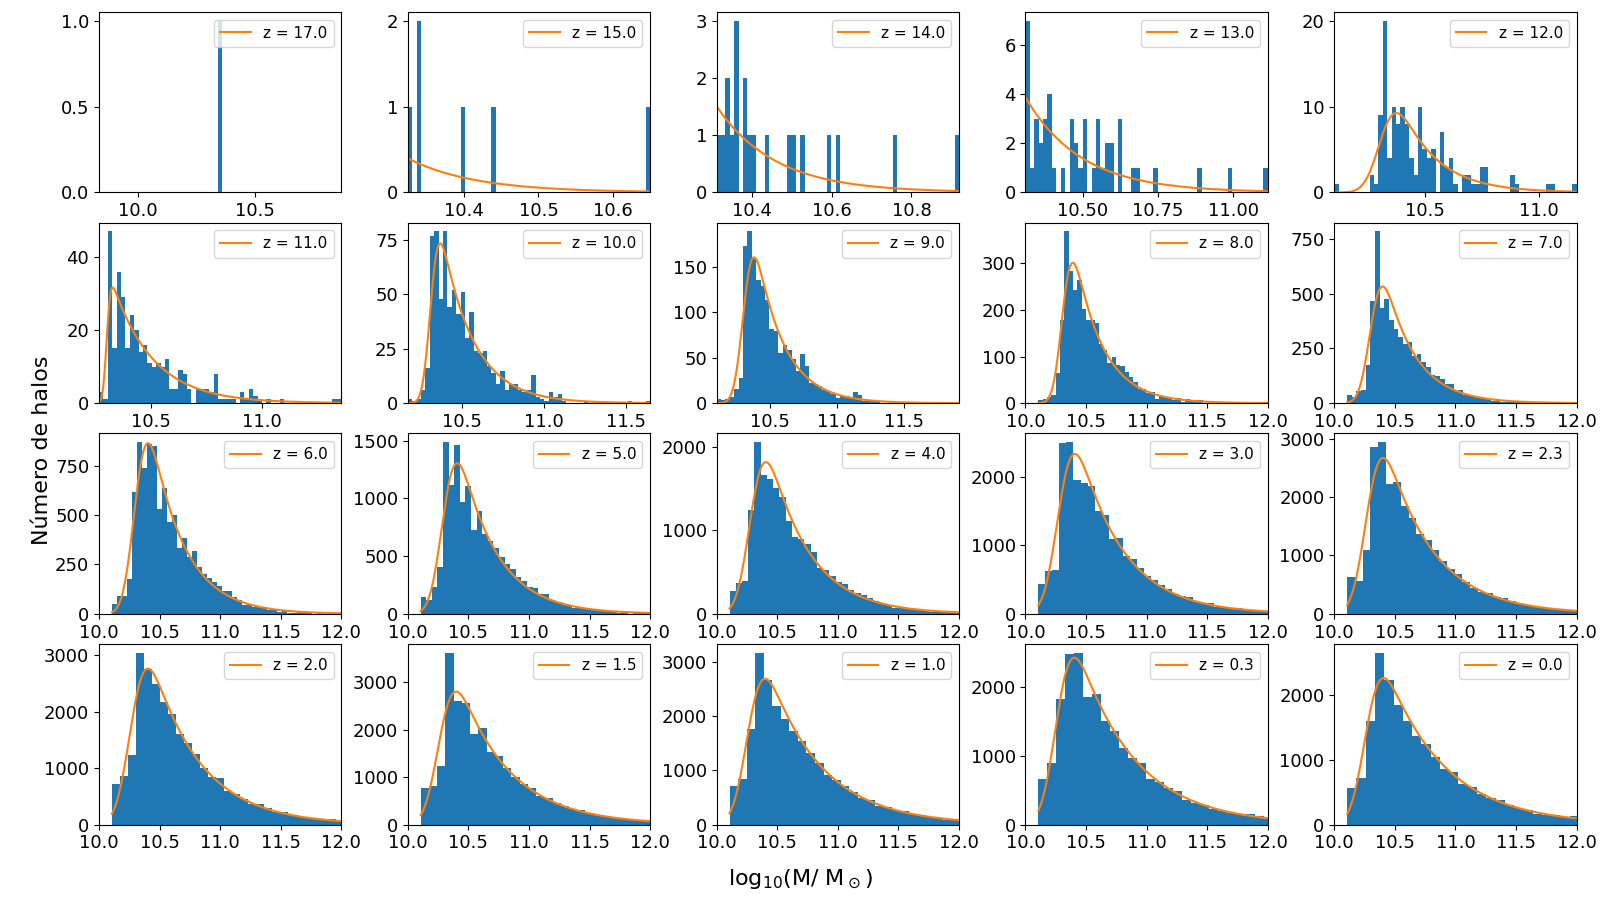
\includegraphics[width = 0.8\linewidth]{RunCanonica/Mass_Dist_RunCanonicaSep.png}
    \caption[Distribución de masa en la evolución de un Universo $\Omega_\lambda = 0.691 $, $\Omega_0 = 0.309$]{\footnotesize Se muestra la distribución de la masa conforme evoluciona el Universo en una cosmología $\Omega_\lambda = 0.691 $ y $\Omega_0 = 0.309$. Se observa como aumentan la cantidad de halos cada vez mas masivos.}
    \label{fig:MassDistCanonRunSep}
\end{figure}

\begin{figure}[ht!]
    \centering
    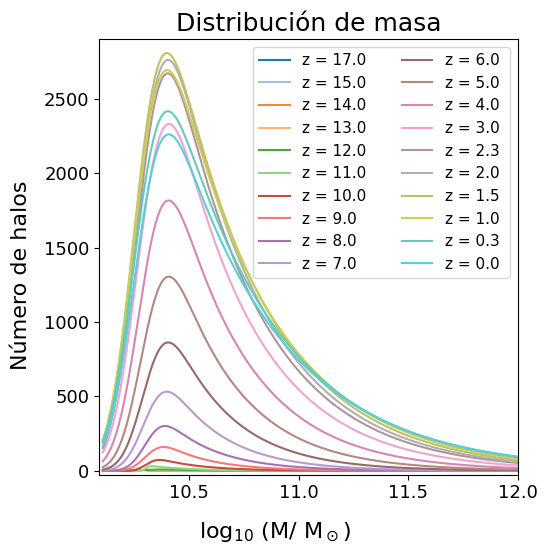
\includegraphics[width = 0.5\linewidth]{RunCanonica/Mass_Dist_RunCanonica.png}
    \caption[Comparación de distribución de masa Universo $\Omega_\lambda = 0.691 $, $\Omega_0 = 0.309$]{\footnotesize Comparación de las distribuciones de masa durante la evolución del Universo $\Omega_\lambda = 0.691 $, $\Omega_0 = 0.309$. Se observa como crece la cantidad de halos de materia oscura, asi como el tamaño de estos.}
    \label{fig:MassDistCanonRun}
\end{figure}

En las figuras \ref{fig:MassDistCanonRun} y \ref{fig:MassStatsCanonRun} podemos apreciar como con el tiempo, los halos de materia oscura se vuelven mas masivos así como vemos un aumento en la variedad de masas que hay. Por lo que en redshifts altos vemos pocas y pequeñas estructuras y en redshifts bajos vemos una mayor cantidad de estructuras con una gran variedad en las masas.

\begin{figure}[ht!]
    \centering
    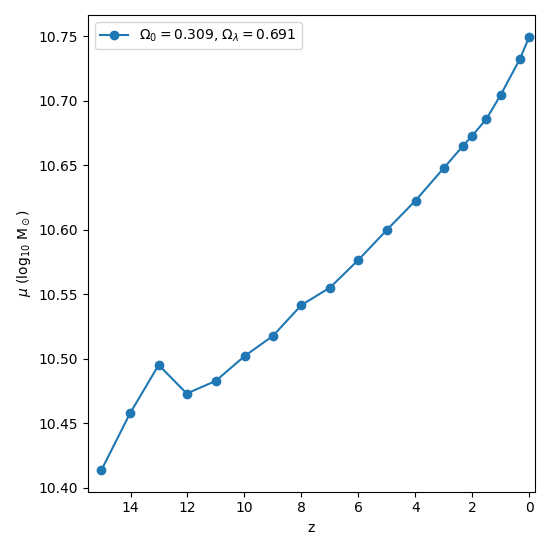
\includegraphics[width = 0.4\linewidth]{RunCanonica/MassMean_RunCanonica.png}
    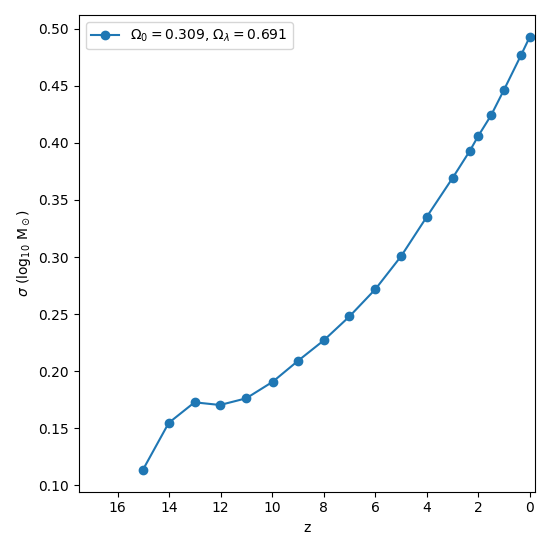
\includegraphics[width = 0.4\linewidth]{RunCanonica/MassStd_RunCanonica.png}
    \caption[Media y desviación estándar de la distribución de masa de un Universo $\Omega_\lambda = 0.691 $, $\Omega_0 = 0.309$]{\footnotesize En la izquierda se muestra la masa media de los halos de materia oscura y se observa como cambia durante la evolución del Universo. En la derecha se muestra la desviación estándar de la masa, la cual nos muestra la variedad que hay de los halos de materia oscura.}
    \label{fig:MassStatsCanonRun}
\end{figure}

Nos hemos dado cuenta de como cambia la distribución de la masa conforme evolucionan el sistema de materia oscura, pero no hemos visto los efectos en los tamaño. Empezando con el radio de la mitad del radio. En las figura \ref{fig:HalfMassRadDistCanonRun} y \ref{fig:HalfMassRadDistCanonRunSep} se observa que el radio crece de manera que en los momentos tempranos tiene un radio entre $10^{0.35}$kpc y $10^{1}$kpc y mas al presente vemos radios entre $10^{5}$kpc y $10^{2.75}$kpc. En la figura \ref{fig:HalfMassRadStatsCanonRun} Observamos con mayor claridad el crecimiento en el radio, siendo que la media va de $10^{0.35}$ kpc a tener radio de $10^{1.5}$kpc. También vemos que hay un aumento en la variedad en los tamaños y además se ve que hay un crecimiento acelerado en la variedad de halos que se observan a lo largo del tiempo.

\begin{figure}[ht!]
    \centering
    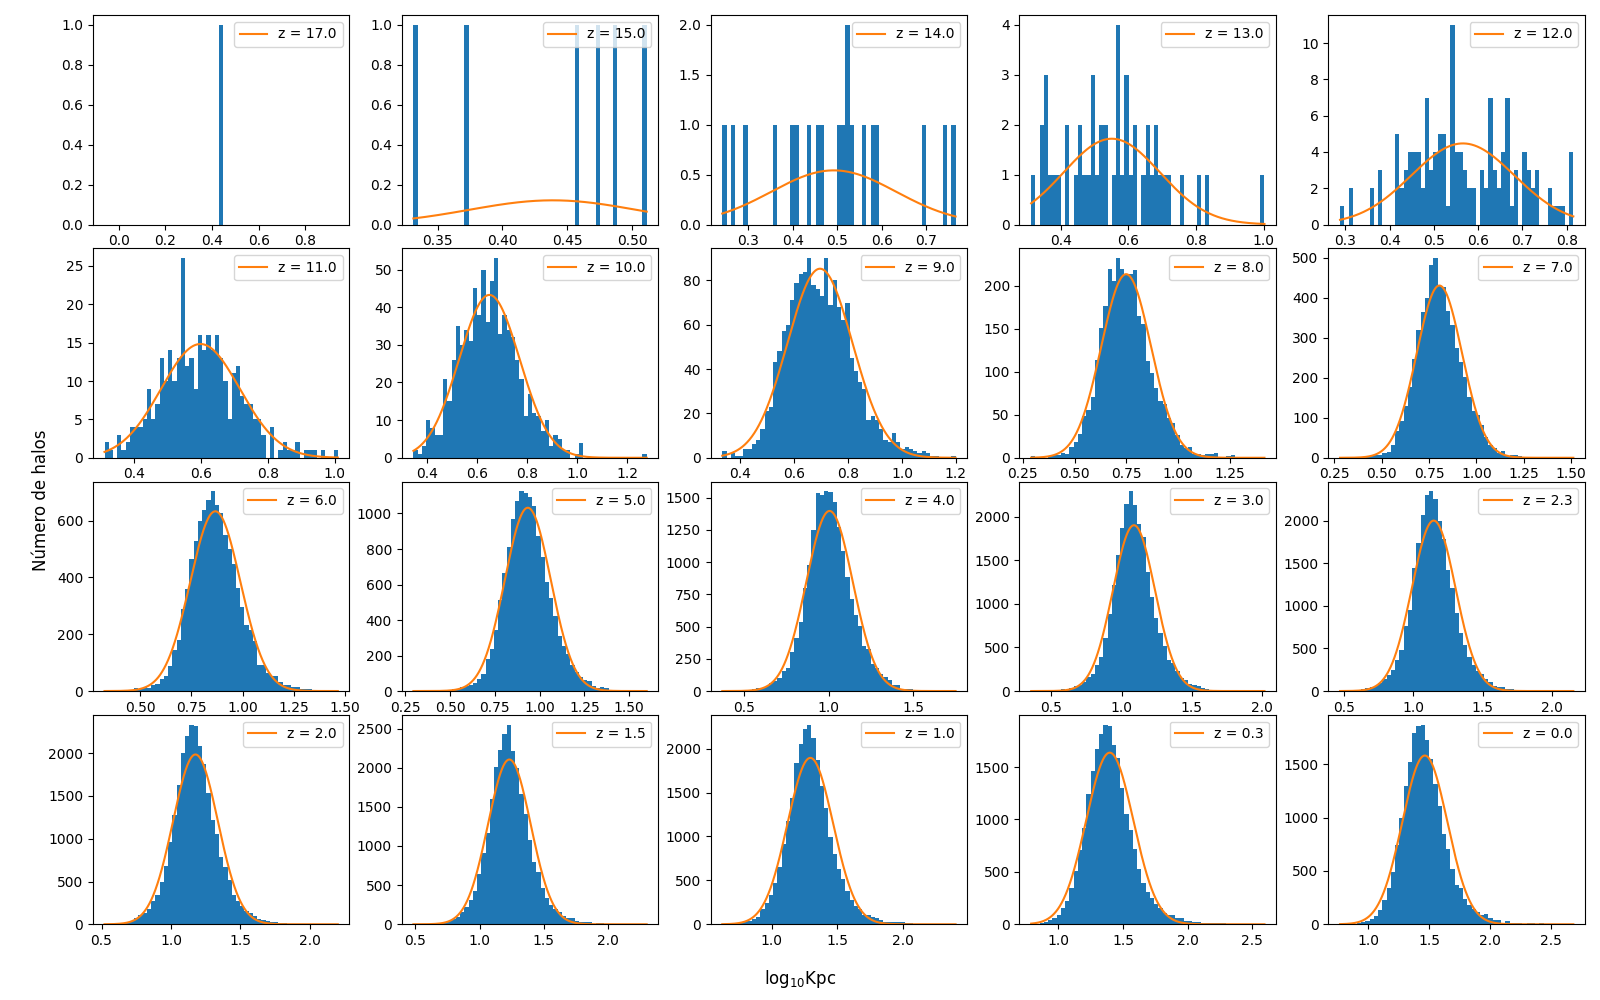
\includegraphics[width = 0.75\linewidth]{RunCanonica/HalfMassRad_Dist_RunCanonicaSep.png}
    \caption[Radio que contiene la mitad de la masa en la evolución de un Universo $\Omega_\lambda = 0.691 $, $\Omega_0 = 0.309$]{\footnotesize Se muestra el radio que contiene la mitad de la masa conforme evoluciona el Universo en una cosmología $\Omega_\lambda = 0.691 $ y $\Omega_0 = 0.309$.}
    \label{fig:HalfMassRadDistCanonRunSep}
\end{figure}

\begin{figure}[ht!]
    \centering
    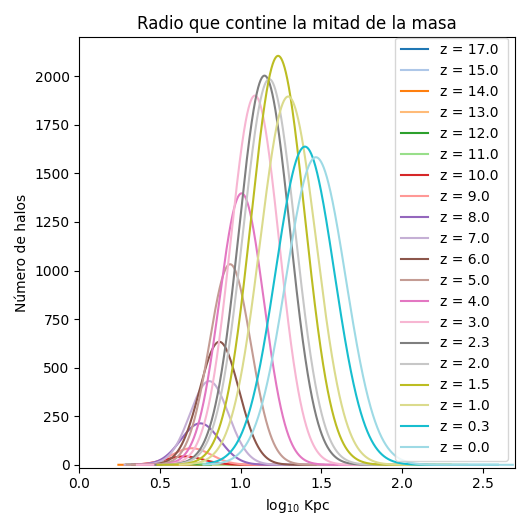
\includegraphics[width = 0.5\linewidth]{RunCanonica/HalfMassRad_Dist_RunCanonica.png}
    \caption[Distribución del Radio que contiene la mitad de la masa de un Universo $\Omega_\lambda = 0.691 $, $\Omega_0 = 0.309$]{\footnotesize Comparación de las distribuciones del radio que contiene la mitad de la masa de los halos de materia oscura de un Universo $\Omega_\lambda = 0.691 $, $\Omega_0 = 0.309$.}
    \label{fig:HalfMassRadDistCanonRun}
\end{figure}

\begin{figure}[ht!]
    \centering
    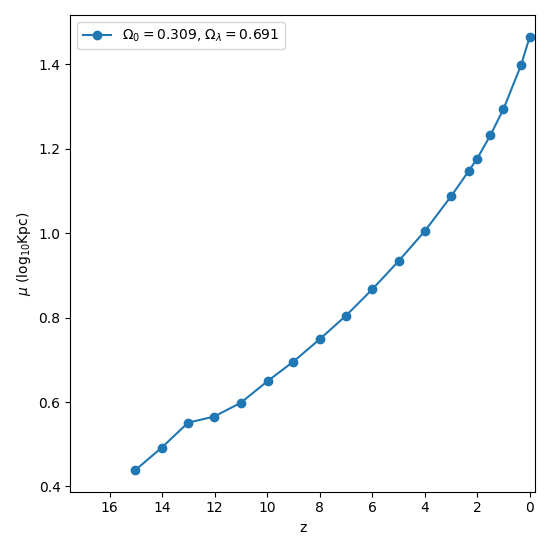
\includegraphics[width = 0.4\linewidth]{RunCanonica/HalfMassRad_Mean_RunCanonica.png}
    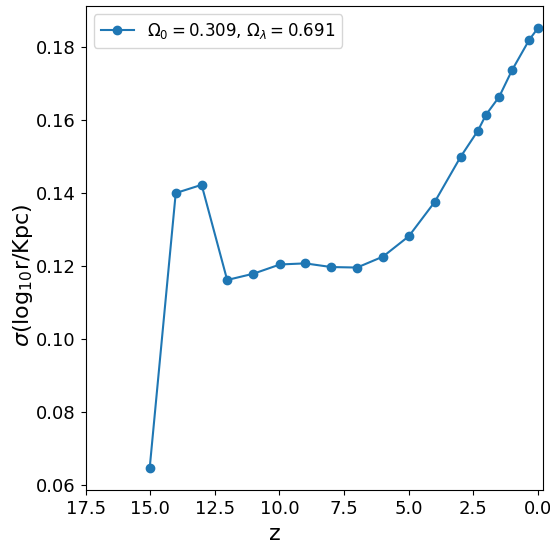
\includegraphics[width = 0.4\linewidth]{RunCanonica/HalfMassRad_Std_RunCanonica.png}
    \caption[Media y desviación estándar del radio de la mitad de la masa de un Universo $\Omega_\lambda = 0.691 $, $\Omega_0 = 0.309$]{\footnotesize En la izquierda mostramos la media del radio que contiene la mitad de la masa de los halos de materia oscura y en la derecha se muestra su desviación estándar a lo largo de la evolución del Universo.}
    \label{fig:HalfMassRadStatsCanonRun}
\end{figure}

Otra medida que utilizamos para dar una idea en el tamaño que tienen los halos es usando el radio donde tenemos la mayor velocidad radial. Las figuras \ref{fig:VMaxRadDistCanonRunSep} y \ref{fig:VMaxRadDistCanonRun} nos muestran la distribución de los radios donde se alcanza la velocidad circular maxima. Podemos ver que con el tiempo, empiezan a verse radios cada vez mas grandes, teniendo estructuras con radios hasta 10 veces mas grandes que la media. La figura \ref{fig:VMaxRadStatsCanonRun} nos muestra el crecimiento medio que tienen los halos a lo largo del tiempo. Aquí se observa un crecimiento acelerado del radio, teniendo las primeras estructuras con radios de $2.45$kpc y las estructuras mas modernas con radios de $27.60$kpc. También observamos que la diversidad de halos aumenta aceleradamente con desviaciones de $0.8$kpc en el pasado hasta $15.7$ kpc



\begin{figure}[ht!]
    \centering
    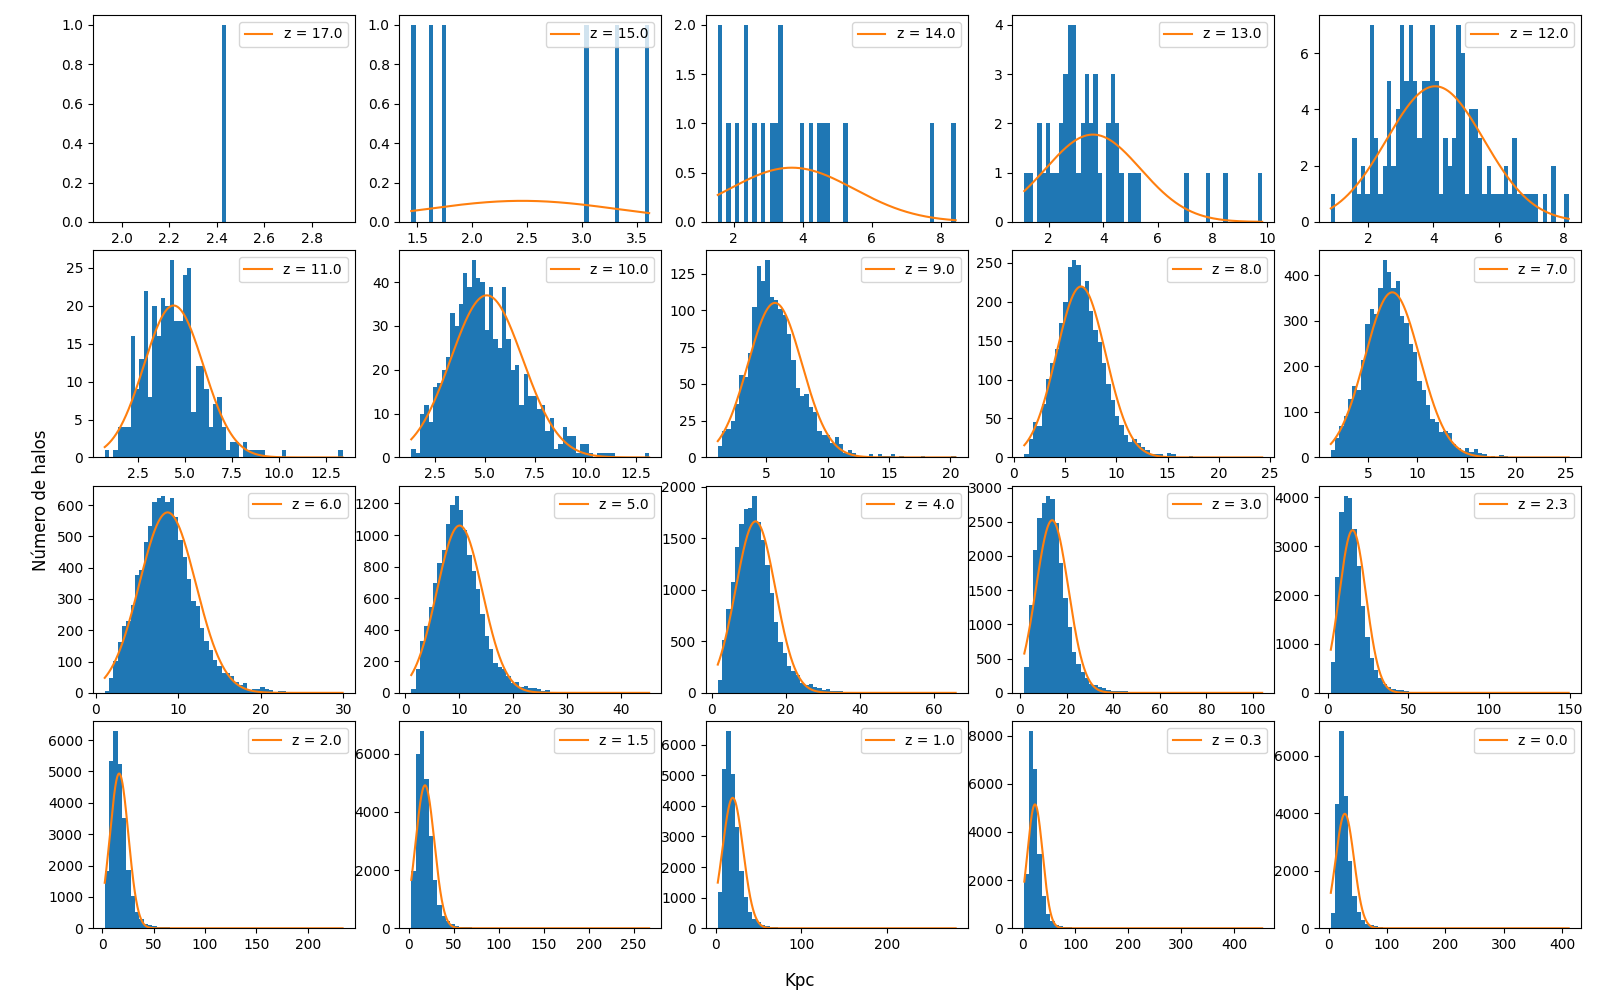
\includegraphics[width = 0.75\linewidth]{RunCanonica/VMaxRad_Dist_RunCanonicaSep.png}
    \caption[Radio donde se alcanza la velocidad maxima radial en la evolución de un Universo $\Omega_\lambda = 0.691 $, $\Omega_0 = 0.309$]{\footnotesize Se muestra el radio donde se alcanza la velocidad maxima radial conforme evoluciona el Universo en una cosmología $\Omega_\lambda = 0.691 $ y $\Omega_0 = 0.309$. Se observa como aumentan la cantidad de halos cada vez mas masivos.}
    \label{fig:VMaxRadDistCanonRunSep}
\end{figure}

\begin{figure}[ht!]
    \centering
    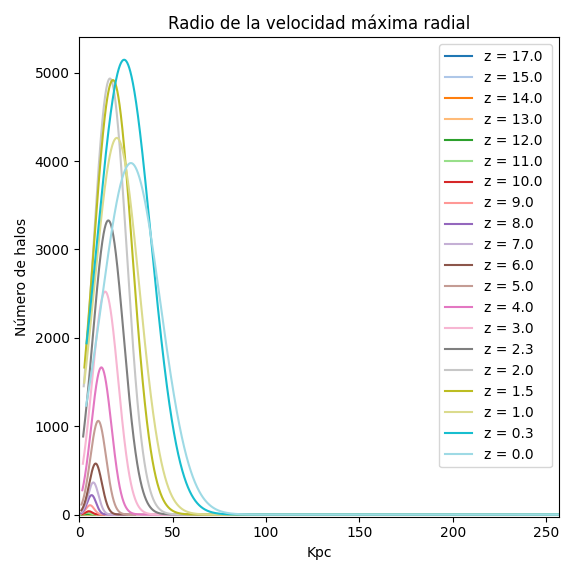
\includegraphics[width = 0.5\linewidth]{RunCanonica/VMaxRad_Dist_RunCanonica.png}
    \caption[Distribución del radio donde se alcanza la velocidad maxima radial de un Universo $\Omega_\lambda = 0.691 $, $\Omega_0 = 0.309$]{\footnotesize Comparación de las distribuciones del radio donde se alcanza la velocidad maxima radial de los halos de materia oscura de un Universo $\Omega_\lambda = 0.691 $, $\Omega_0 = 0.309$.}
    \label{fig:VMaxRadDistCanonRun}
\end{figure}


\begin{figure}[ht!]
    \centering
    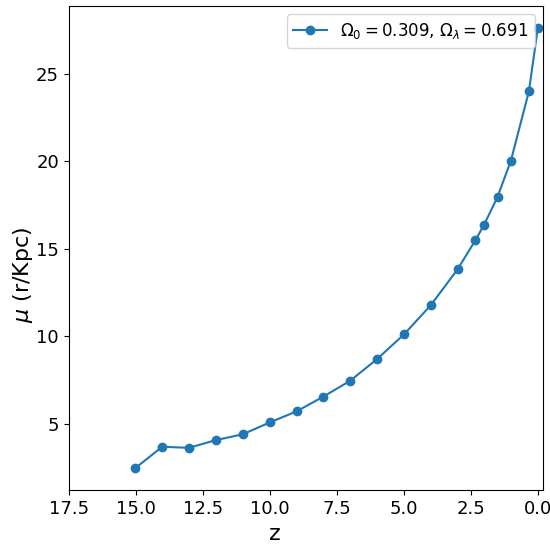
\includegraphics[width = 0.4\linewidth]{RunCanonica/VMaxRad_Mean_RunCanonica.png}
    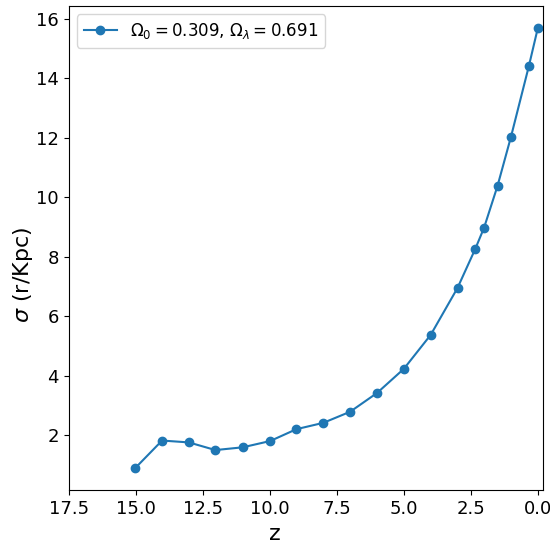
\includegraphics[width = 0.4\linewidth]{RunCanonica/VMaxRad_Std_RunCanonica.png}
    \caption[Media y desviación estándar del Radio de la mitad de la masa de un Universo $\Omega_\lambda = 0.691 $, $\Omega_0 = 0.309$]{\footnotesize En la izquierda mostramos la media del radio donde se alcanza la velocidad maxima radial de los halos de materia oscura y en la derecha se muestra su desviación estándar a lo largo de la evolución del Universo.}
    \label{fig:VMaxRadStatsCanonRun}
\end{figure}



La figura \ref{fig:CanonRunDensityMap} podemos observar a lo que conocemos como la \emph{Cosmic Web}. Se observa la simulación desde un plano, donde tenemos varias imágenes que muestran el cambio con el tiempo. En les redshift altos se observan nubes difusas donde no se alcanza a visualizar gran estructura, mientras que los redshift bajos, se observan objetos mejor definidos y en grandes cantidades.


\begin{figure}[ht!]
    \centering

    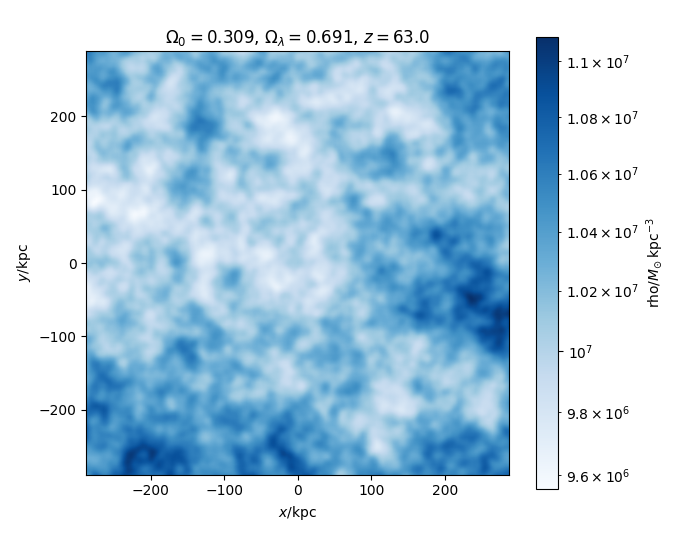
\includegraphics[width = 0.33\linewidth]{RunCanonica/RunCanonZ63Rho.png}   %snap 000
    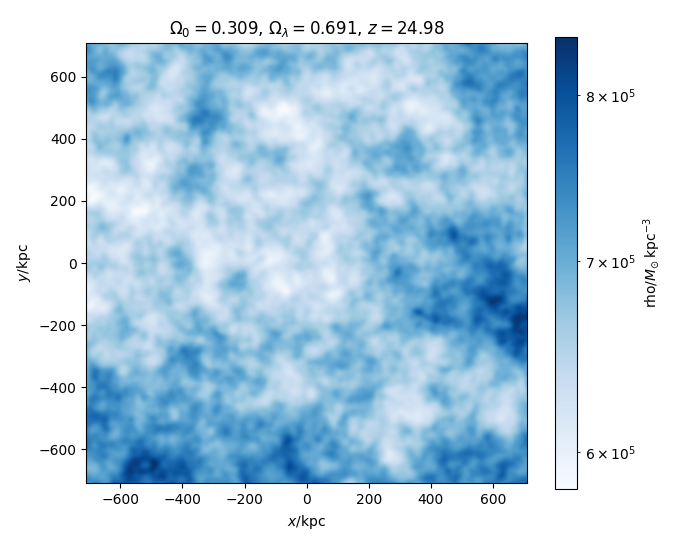
\includegraphics[width = 0.33\linewidth]{RunCanonica/RunCanonZ25Rho.png}   %snap 005
    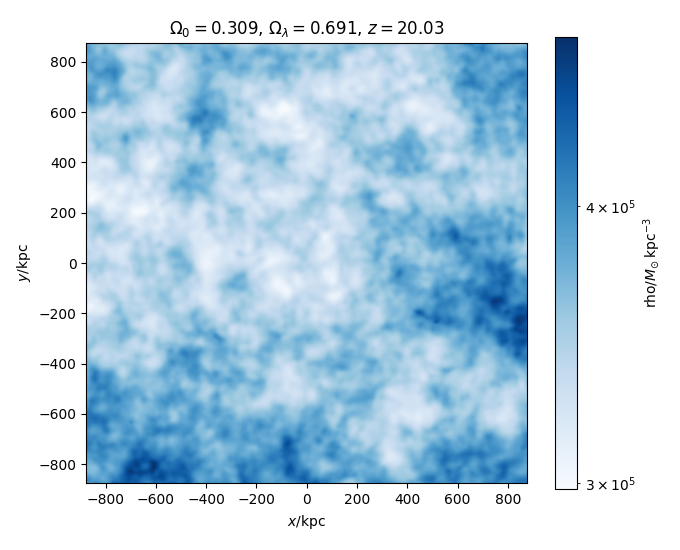
\includegraphics[width = 0.32\linewidth]{RunCanonica/RunCanonZ20Rho.png}   %snap 010
    \\
    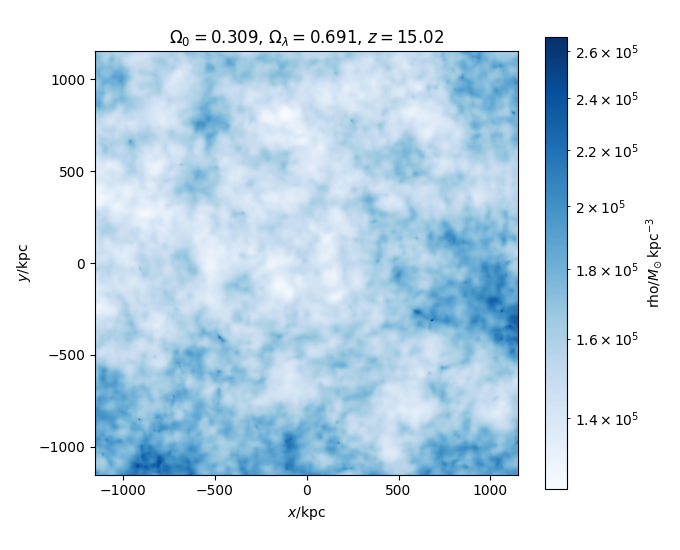
\includegraphics[width = 0.33\linewidth]{RunCanonica/RunCanonZ15Rho.png}   %snap 015
    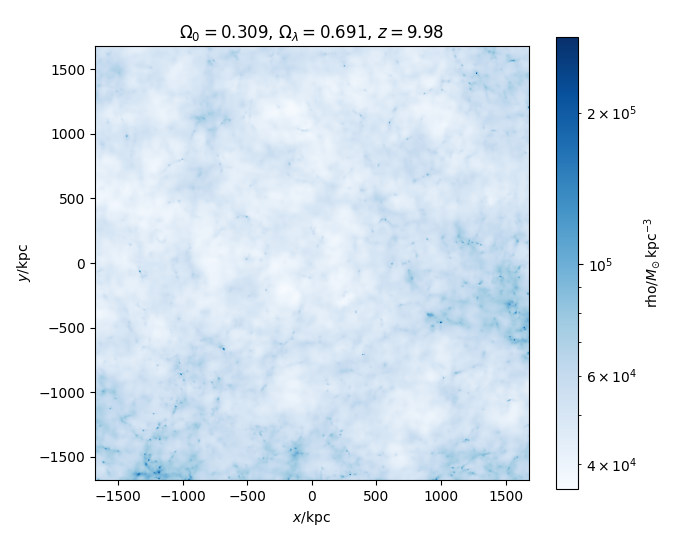
\includegraphics[width = 0.33\linewidth]{RunCanonica/RunCanonZ10Rho.png}   %snap 020
    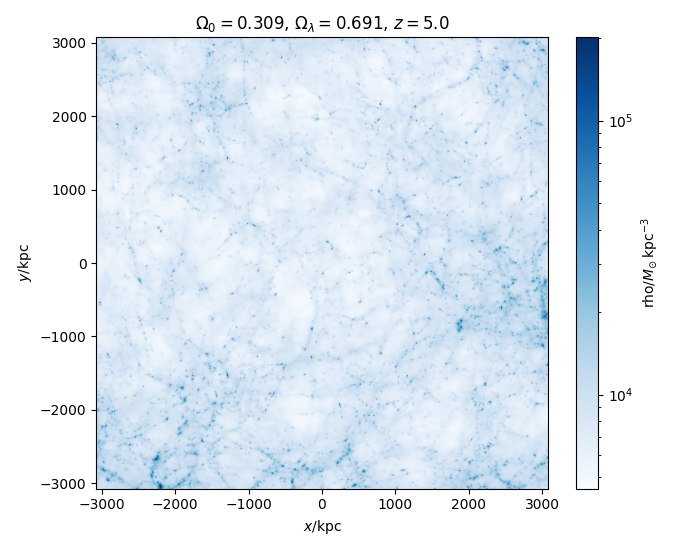
\includegraphics[width = 0.32\linewidth]{RunCanonica/RunCanonZ5Rho.png}    %snap 025
    \\
    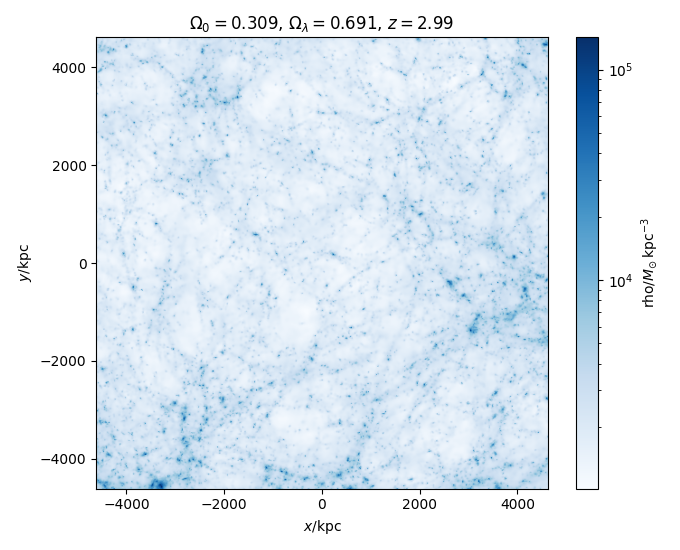
\includegraphics[width = 0.33\linewidth]{RunCanonica/RunCanonZ3Rho.png}    %snap 027
    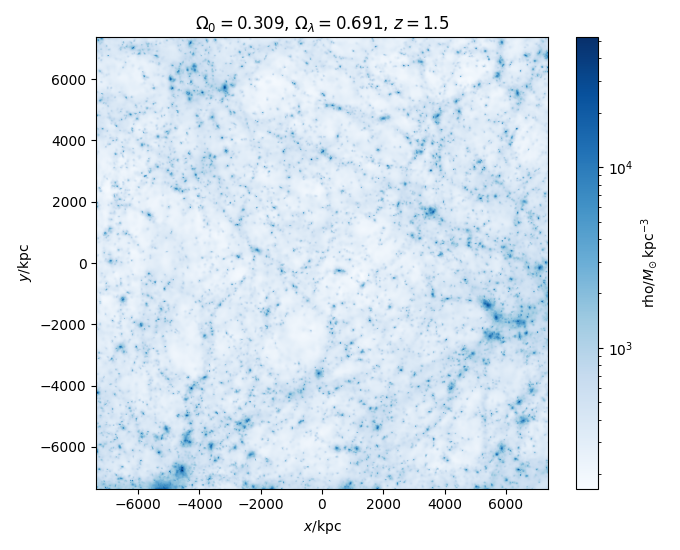
\includegraphics[width = 0.33\linewidth]{RunCanonica/RunCanonZ1_5Rho.png}  %snap 030
    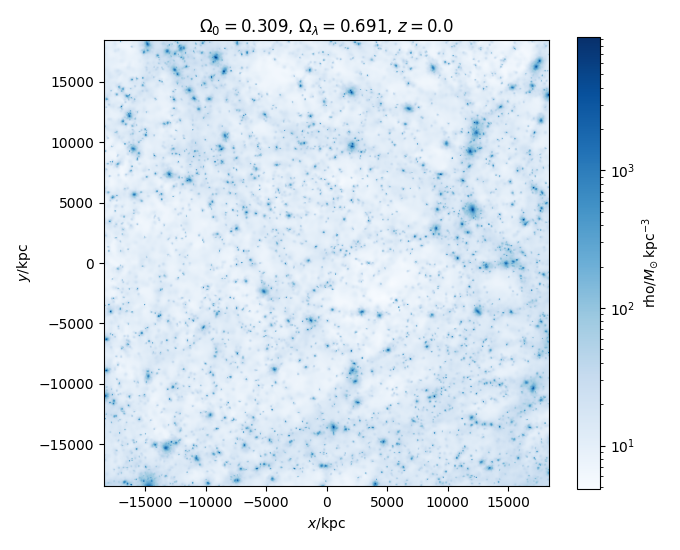
\includegraphics[width = 0.32\linewidth]{RunCanonica/RunCanonZ0Rho.png}    %snap 033
    \caption[Mapa de densidad de un Universo $\Omega_\lambda = 0.691 $, $\Omega_0 = 0.309$ en en diferentes redshift]{ \footnotesize Mapa de densidad de la simulación en diferentes redshifts de una cosmología $\Omega_\lambda = 0.691 $, $\Omega_0 = 0.309$. }
    \label{fig:CanonRunDensityMap}
\end{figure}








\subsection{ Universo con cosmología  \texorpdfstring{$\Omega_\lambda = 0.691$, $\Omega_0 = 0.309$ }{Omega lambda = 0.691, Omega 0 = 0.309} }


